\chapter*{Proyecto sector Arduino} 
%
\addtocounter{ns}{1} 
\section{Introducción}

El proyecto de extensión EDETEC, tiene una unidad, denominada sector Arduino. Este sector, fomenta el desarrollo, utilizando esta plataforma de software y hardware libre. Todos los años, se forman técnicos en electrónica provenientes de la escuela Albert Thomas, ubicada en calle 1 esq 57, en la ciudad de La Plata. Esta formación, corresponde a la materia denominadas ``prácticas profesionalizantes'', donde los alumnos, trabajan en algún desarrollo libre, relacionado a las temáticas del laboratorio. La modalidad de trabajo, a partir del año 2018 es la siguiente: 
\begin{enumerate}
	\item Generar tormenta de ideas.
	\item Elegir uno de las ideas propuestas anteriormente.
	\item Crear especificaciones sobre la propuesta (o comúnmente denominados requerimientos, en su mayor parte son de tipo L1).
	\item Realizar el plan de acción para llevar a cabo la propuesta a lo largo del ciclo lectivo.
\end{enumerate}

El presente año, se ha presentado la propuesta de crear un bastón inteligente para personas con capacidad visual reducida. 

\section{Bastón inteligente}

El bastón inteligente, se ha propuesto, basado en una idea, obtenida a partir de una nota periodistica, de un medio extranjero. Este, bastón, debe realizar las siguientes tareas: 
\begin{enumerate}
	\item Detectar ubicación (dirección)  
	\item Medir distancias a posibles obstáculos
	\item Uso a baterías. Estas, serán recargables con algún puerto USB o micro USB. 
	\item Avisar mediante voz, o alarmas, si tiene un posible obstáculo cerca
\end{enumerate}

La realización de este proyecto, implica crear un prototipo,
que luego, se debe verificar con algún usuario que posea capacidad visual reducida, y ser probado, y en base a eso, ajustar los resultados del prototipo. El bastón, responderá al siguiente esquema. 
\begin{figure}[ht!]
	\hspace{-2.5cm}
	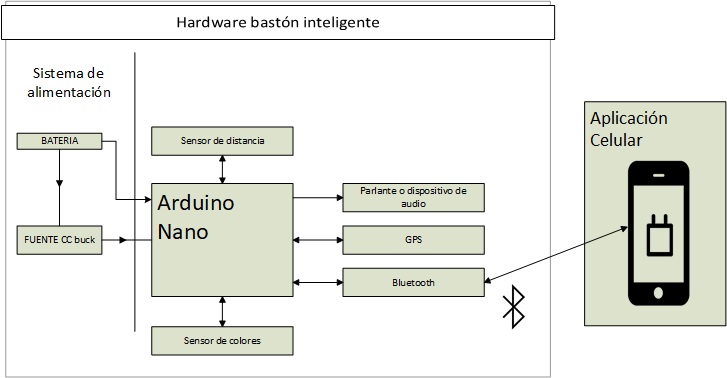
\includegraphics{images/diagrama_baston_inteligente.png} 
	\caption{Diagrama en bloques del sistema a implementar}
\end{figure}

Como se observa, en esta figura, el sistema posee un microcontrolador, el cual tiene un código, que esta disponible para su consulta en el sistema de repositorios GitHub. En caso de necesitar su acceso, contactarse con alguno de los autores del presente documento. Este actualmente, se encuentra en privado, y se mantendrá de esta forma, hasta terminar el código en su totalidad. 

\section{Proyecto y estado de avance}


Como se ha dicho, en la primera sección, se debe realizar un plan de acción, para poder lograr el objetivo con éxito. El proyecto, se ha dividido en tres fases. Las mismas se muestran en la siguiente tabla, en conjunto con sus tareas.  

\begin{table}[ht!]
	\centering
	\begin{tabular}{|c|c|c|}
		\hline 
		Fase & Tarea & estado de avance[\%] \\ 
		\hline 
		\multirow{3}{4cm}{Fase de análisis} & Análisis de componentes & 100 \\ \cline{2-3}   
		&  Requerimientos del proyecto &100 \\ \cline{2-3}   
		&  Análisis de costo &  100 \\  \hline
		\multirow{3}{4cm}{Fase de diseño} & Diagrama de software y hardware & 100 \\  \cline{2-3}
		&Desarrollo de funcionalidad & 80  \\ \cline{2-3} 
		&Integración de software y hardware & 20  \\ \cline{2-3} 
		&Verificación de software y hardware & 20  \\ \hline 
		\multirow{3}{4cm}{Fase de resultados} & simulación & 30\\  \cline{2-3}
		&Creación de prototipo& 5     \\  \cline{2-3}
		&Resultados y conclusiones& 0 \\  \cline{2-3}
		&Generación de documentación & 8 \\ \hline 		
	\end{tabular}
\caption{Plan de acción del proyecto bastón inteligente perteneciente al sector arduino}
\end{table}



 

